\section{Reduction From \bmhpc to Degeneracy}\label{sec:reduction}

In this section we prove streaming lower bounds for degeneracy related problems. Precisely, we prove the following theorem. 
\begin{restatable}{theorem}{mainthmdegen}
\label{thm:degen-lb}
Given an integer $k$ and an $n$-vertex graph $G$, any $p$-pass streaming algorithm that can check whether $\kappa(G)\leq k$ or not requires $\Omega(n^2/p^3- (n\log n)/p)$ space.   \end{restatable}

This immediately implies the following corollary for semi-streaming algorithms.

\begin{corollary}
A semi-streaming algorithm for any of the following problems on an $n$-vertex graph $G$ requires $\tilde{\Omega}(n^{1/3})$ passes.
\begin{itemize}
    \item Check whether the degeneracy $\kappa(G)\leq k$ for a given integer $k$.
    \item Exactly compute the value of  $\kappa(G)$.
    \item Find a degeneracy ordering of $G$.
    \item Find a non-empty $k$-core of $G$ for a given value of $k$ (or report NONE if none exists).
\end{itemize}
 \end{corollary}


We prove \Cref{thm:degen-lb} by reduction from \bmhpc. Suppose we are given an instance of $\bmhpc_{m,r}$. We first describe a gadget graph $G$ based on this instance, and prove that this graph's degeneracy $\kappa(G)$ being $\leq k$ or $>k$ (for some particular value $k$) can be used to determine whether the solution to the \bmhpc instance is $0$ or $1$. Then, along standard lines, we show how a streaming algorithm that solves this boolean version of the  degeneracy problem can be used to design a communication protocol for $\bmhpc_{m,r}$, implying that the space used by the streaming algorithm must be at least the communication complexity of $\bmhpc_{m,r}$. 

\subsection{Construction of the Gadget Graph}\label{sec:redn-graph}
 In \Cref{fig:graph-const}, we show the graph constructed for a particular instance of \bmhpc. We then formally describe the construction and refer to the figure for examples. 
 
\begin{figure}[H]
\centering
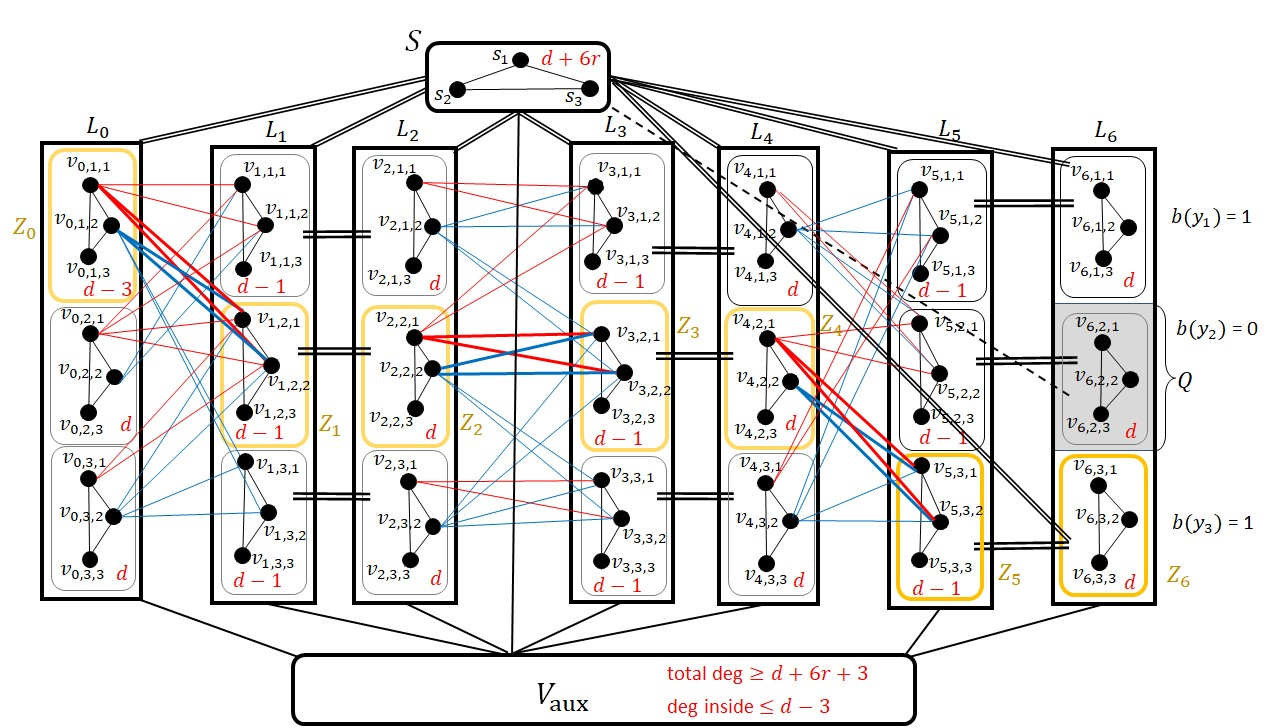
\includegraphics[scale=0.6]{figures/fig1}
\caption{\small The gadget graph $G$ for the following instance of $\bmhpc_{3,3}$. $\bfA^1 = \{A^1_{x_1} = \{y_1,y_2\}, A^1_{x_2} = \{y_1,y_2\}, A^1_{x_3} = \{y_2\}\}$. $\bfB^1 =\{ B^1_{x_1} = \{y_2, y_3\}, B^1_{x_2} = \{y_1\}, B^1_{x_3} = \{y_2, y_3\}\}$. $\bfC^2= \{C^2_{y_1} = \{x_1\}, C^2_{y_2} = \{x_1,x_2\}, C^2_{y_3} = \{x_3\}\}$. $\bfD^2 = \{D^2_{y_1} = \{x_1,x_2\}, D^2_{y_2} = \{x_2,x_3\}, D^2_{y_3} = \{x_2,x_3\}\}$. $\bfA^3 = \{A^3_{x_1} = \{y_2\}, A^3_{x_2} = \{y_2,y_3\}, A^3_{x_3} = \{y_1\}\}$. $\bfB^3 =\{ B^3_{x_1} = \{y_1, y_2\}, B^3_{x_2} = \{y_3\}, B^3_{x_3} = \{y_1, y_3\}\}$ (we skip $\bfC^1,\bfD^1,\bfA^2,\bfB^2,\bfC^3,\bfD^3$ because they are redundant). Hence, $z_0=x_1$; $z_1=t^1_{x_1}=y_2$; $z_2=t^2_{y_2}=x_2$; and $z_3=t^3_{x_2}=y_3$. Therefore, the answer to this instance is $b(y_3)=1$.\\
Here, a double line between two sets of nodes (e.g., the one between sets $S$ and $L_0$) signifies that all possible cross edges are present between those two sets. A single line between two sets (e.g., the one between $\Vaux$ and $L_0$) denotes that some edges maybe present between them. A dashed line (e.g., the one between sets $S$ and $Q$) denotes that absolutely no edge is present between them. For each triple, the number (in red) inside the box containing it denotes the degree of each node in the triple. The red and blue edges encode the inputs. The thick edges are between triples representing $z_i$ and $z_{i+1}$.}
\label{fig:graph-const}
\end{figure}

 The graph $G$ has $2r+1$ {\em layers} $L_0, L_1, \ldots L_{2r}$. Each layer $L_{\ell}$ has $3m$ nodes. Edges between two of these layers are always between successive layers $L_{\ell}$ and $L_{\ell+1}$ for some $\ell$.

 \mypar{Layer nodes} For each $\ell \in [0,2r]$ and for each $i\in [m]$, layer $L_\ell$ has $3$ nodes (a \emph{triple}), denoted by $v_{\ell,i,1}, v_{\ell,i,2}$, and $v_{\ell,i,3}$. For $\ell=0$, this triple represents $x_i$. For $\ell\geq 0$, in layers $L_{4\ell+1}$ and $L_{4\ell+2}$ (resp. $L_{4\ell+3}$ and $L_{4\ell+4}$), it represents $y_i$ (resp. $x_i$). For instance, in \Cref{fig:graph-const}, the triple $(v_{3,2,1}, v_{3,2,2},v_{3,2,3})$ represents $x_2$ and $(v_{6,1,1}, v_{6,1,2},v_{6,1,3})$ represents $y_1$. Formally, we add the following set of vertices. $$V_L = \left\{v_{\ell,i,c}:\ell\in [0,2r], i\in [m], c\in \{1,2,3\}\right\}$$
 
 
 \mypar{Special nodes} Outside the layers, we have a set $S$ of three special nodes $s_1, s_2, s_3$. 

\smallskip
We now define the edges on the node set $V_L\cup S$.

 \mypar{Edges within each triple} Each triple forms a triangle. Formally, we add the edge set $E_1$ to $G$, where 
$$E_1=\left\{(v_{\ell, i,1}, v_{\ell, i,2}), (v_{\ell, i,2}, v_{\ell, i,3}), (v_{\ell, i,1}, v_{\ell, i,3}): \ell\in [0,2r], i\in [m] \right\}$$


\mypar{Edges between layers $L_{2\ell-1}$ and $L_{2\ell}$} As mentioned above, for each $\ell\in [r]$, either both of the $i$th triples in layers $L_{2\ell-1}$ and $L_{2\ell}$ represent $x_i$ or both represent $y_i$. We add all $9$ cross edges between these two triples representing the same element. E.g., in \Cref{fig:graph-const}, we have all cross edges (denoted by a double line) between the triples $(v_{1,1,1}, v_{1,1,2}, v_{1,1,3})$ and $(v_{2,1,1}, v_{2,1,2}, v_{2,1,3})$, both of which represent $y_1$. Formally, we add the edge set $E_2$ to $G$, where 
$$E_2=\left\{\left\{v_{2\ell-1, i, c}: c\in \{1,2,3\}\right\}\times \left\{v_{2\ell, i, c}: c\in \{1,2,3\}\right\}: \ell\in [r], i\in [m] \right\}$$

\mypar{Edges between layers $L_{4\ell}$ and $L_{4\ell+1}$} The edges connecting layers of the form $L_{4\ell}$ and $L_{4\ell+1}$ encode the inputs $\bfA^{2\ell+1}$ and $\bfB^{2\ell+1}$. In particular, for each $i\in [m]$, the edges leaving $v_{4\ell, i, 1}$ and $v_{4\ell, i, 2}$ encode the sets $A_{x_i}^{2\ell+1}$ and $B_{x_i}^{2\ell+1}$ respectively. Precisely, if the set $A_{x_i}^{2\ell+1}$ contains the element $y_j$, then we join $v_{4\ell, i, 1}$ to both the nodes $v_{4\ell+1, j, 1}$and $v_{4\ell+1, j, 2}$. Similarly, if $B_{x_i}^{2\ell+1}$ contains $y_j$, then we join $v_{4\ell, i, 2}$ to both $v_{4\ell+1, j, 1}$ and  $v_{4\ell+1, j, 2}$ (for example, see the families ($\bfA^1$,$\bfB^1$) and ($\bfA^3$,$\bfB^3$) in \Cref{fig:graph-const}, and the corresponding edges between $L_0$ and $L_1$ and between $L_4$ and $L_5$ respectively). Formally, we add the edge sets $E_A$ and $E_B$ to $G$, where 


\begin{itemize}
\item $E_A= \left\{\left\{v_{4\ell, i, 1}\right\}\times \left\{v_{4\ell+1,j,1}, v_{4\ell+1, j, 2}\right\}: y_j\in A_{x_i}^{2\ell+1}, \ell\in [0,\floor{(r-1)/2}], j\in [m]\right\}$

\item $E_B= \left\{\left\{v_{4\ell, i, 2}\right\}\times \left\{v_{4\ell+1,j,1}, v_{4\ell+1, j, 2}\right\}: y_j\in B_{x_i}^{2\ell+1}, \ell\in [0,\floor{(r-1)/2}], j\in [m]\right\}$
\end{itemize}

\mypar{Edges between layers $L_{4\ell+2}$ and $L_{4\ell+3}$} The edges between layers of the form $L_{4\ell+2}$ and $L_{4\ell+3}$ similarly encode the inputs $\bfC^{2\ell+2}$ and $\bfD^{2\ell+2}$. The construction is same as above, except with $A_{x_i}^{2\ell+1}$ and $B_{x_i}^{2\ell+1}$ replaced by $C_{y_i}^{2\ell+2}$ and $D_{y_i}^{2\ell+2}$ respectively, and $y_j$ replaced by $x_j$ (again, see the families $\bfC^2$ and $\bfD^2$ in the example in \Cref{fig:graph-const} and the corresponding edges between $L_2$ and $L_3$). Formally, we add the edge sets $E_C$ and $E_D$ to $G$, where

\begin{itemize}
\item $E_C= \left\{\left\{v_{4\ell+2, i, 1}\right\}\times \left\{v_{4\ell+3,j,1}, v_{4\ell+3, j, 2}\right\}: x_j\in C_{y_i}^{2\ell+2}, \ell\in [0,\floor{r/2}-1], j\in [m]\right\}$

\item $E_D= \left\{\left\{v_{4\ell+2, i, 2}\right\}\times \left\{v_{4\ell+3,j,1}, v_{4\ell+3, j, 2}\right\}: x_j\in D_{y_i}^{2\ell+2}, \ell\in [0,\floor{r/2}-1], j\in [m]\right\}$
\end{itemize}

\mypar{Edges on special nodes} Recall that each element in $\cX$ and $\cY$ has a bit associated with it. The special nodes $s_1,s_2,s_3$ are connected to each other and also to all the layer nodes except those representing bit-$0$-elements in the last layer $L_{2r}$ (in  \Cref{fig:graph-const}, this is the triple representing $y_2$ in $L_6$). Formally, if $r$ is even, let $Q := \left\{v_{2r, i, c}: b(x_i) = 0,~c\in \{1,2,3\}\right\}$, and otherwise, $Q := \left\{v_{2r, i, c}: b(y_i) = 0,~c\in \{1,2,3\}\right\}$. Then, we add the edge set $E_S$ to $G$, where 
$$E_S=\{(s_1,s_2), (s_2,s_3), (s_1,s_3)\}\cup \left(\{s_1, s_2, s_3\}\times (V_L \setminus Q)\right)$$

Let $V' := V_L \cup S$ and $E' := E_1\cup E_2 \cup E_S\cup E_A\cup E_B \cup E_C\cup E_D$. The graph constructed so far is $G'=(V',E')$.

\mypar{Auxiliary edges} We add some auxiliary vertices $\Vaux$ and edges $\Eaux \subseteq \Vaux\times(V'\cup \Vaux)$ to obtain the final graph 
$$G=\left(V' \cup V_{\text{aux}}, E' \cup E_{\text{aux}} \right)$$

\noindent
where we ensure the following degrees for $d:=6mr+3m$ (in \Cref{fig:graph-const}, these degrees are written in the boxes containing the triples). 

\begin{itemize}
    \item $\deg(v_{0,1,1})= \deg(v_{0,1,2}) = \deg(v_{0,1,3}) = d-3$ 
   \item For each $i\in [2,m]$, $c\in\{1,2,3\}$, $\deg(v_{0,i,c})=d$.
   \item For each $\ell\in [r], i\in [m], c\in \{1,2,3\}$, $\deg(v_{2\ell-1,i,c})=d-1$.
    \item For each $\ell\in [r], i\in [m], c\in \{1,2,3\}$, $\deg(v_{2\ell,i,c})=d$.
    \item $\deg(s_1)=\deg(s_2)=\deg(s_3)=d+6r$
    \item For each $u\in \Vaux$, $\deg(u)\geq d+6r+3$. 
\end{itemize}

\Cref{lem:redn-aux-constr} states that such a construction of $\Vaux$ and $\Eaux$ is possible with just the knowledge of the vertex degrees in $G'$ (rather than the actual graph). We shall use this fact in our reduction. The proof with the explicit construction is deferred to \Cref{app:proof-auxnode-redn}.

\begin{lemma}\label{lem:redn-aux-constr}
 Given the degree of each node in $G'=(V',E')$, we can add vertices $V_{\text{aux}}$ and edges $E_{\text{aux}}\subseteq \Vaux \times (V'\cup \Vaux)$ so that the graph $G=\left(V' \cup V_{\text{aux}}, E' \cup E_{\text{aux}}\right)$ has the above vertex-degrees and $\Theta(mr)$ nodes in total. Furthermore, the degree of any vertex in the induced subgraph $G[\Vaux]$ is $\leq d-3$.
\end{lemma}



This completes the construction of the graph $G$. 

\subsection{The Analysis}

In this section, we prove the following lemma that says that we can use the degeneracy value of the gadget graph constructed in the last section to determine the solution to the corresponding instance of \bmhpc. 

\begin{lemma}\label{lem:redn-degen-yesno}
     Given an instance of $\bmhpc_{m,r}$, let $G$ denote the gadget graph constructed in \Cref{sec:redn-graph}. If $b(z_r)=0$, then $\kappa(G)\geq d-2$. Otherwise, $\kappa(G)\leq d-3$.
\end{lemma}

We set up some notations to prove the above lemma.

\mypar{Triples corresponding to pointers} We are particularly interested in the triples of nodes that represent the pointers $z_i$ in the relevant layers. In layer $L_0$, we are interested in the triple representing the first pointer $z_0$; call it $Z_0$. Then in \emph{each} of the layers $L_1$ and $L_2$, we are interested in the triple representing the second pointer $z_1$; call these triples $Z_1$ and $Z_2$ respectively. In general, in layers $L_{2\ell-1}$ and $L_{2\ell}$, the triples that represent the pointer $z_\ell$ are called $Z_{2\ell-1}$ and $Z_{2\ell}$ respectively. In other words, the triple $Z_{\ell}$ corresponds to the pointer $z_{\ceil{\ell/2}}$ (see \Cref{fig:graph-const} for example. $Z_0$ is the triple representing $z_0=x_1$; both $Z_1$ and $Z_2$ represent $z_1=y_2$; both $Z_3$ and $Z_4$ represent $z_2=x_2$; and finally both $Z_5$ and $Z_6$ represent $z_3=y_3$.)

Let us now formalize this. Define the function $i^*:[0,2r]\to [m]$ as follows:

For $\ell\in [0,2r]$, let $\ell' := \ceil{\ell/2}$. Then $i^*(\ell)$ is the unique index $i$ such that 
$$z_{\ell'}= 
\begin{cases}
x_{i} & \text{if $\ell'$ is even}\\
y_{i} & \text{if $\ell'$ is odd}
\end{cases}
$$

Then $Z_\ell:= (v_{\ell,i^*(\ell),1}, v_{\ell,i^*(\ell),2},v_{\ell,i^*(\ell),3})$, i.e., the triple representing $z_{\ceil{\ell/2}}$ in layer $L_\ell$.

\mypar{High-level proof overview} To prove \Cref{lem:redn-degen-yesno}, we perform the peeling algorithm on the graph $G$. We shall show that the first $6r+3$ iterations of this algorithm basically chase the hidden pointers over the successive layers: to be precise, the first three iterations remove the triple $Z_0$, the next three remove $Z_1$, and so on and so forth until iterations $6r+1,6r+2$, and $6r+3$ remove $Z_{2r}$ (see \Cref{fig:first-iter,fig:odd-layer-rem,fig:even-layer-rem} for a sketch of how this proceeds). Then we have two cases as follows. 

If $b(z_r)=0$, then removal of $Z_{2r}$ does not reduce the degrees of the nodes in $S$. We show that in this case, immediately after the removal of $Z_{2r}$, the peeling algorithm must remove a node with degree $\geq d-2$ (\Cref{fig:nocase}). Thus, by \Cref{fact:peelingmin-degen}, we must have $\kappa(G)\geq d-2$.

Otherwise, if $b(z_r)=1$, then $Z_{2r}$ is indeed connected to the nodes $s_1,s_2,s_3$. We show that removal of $Z_{2r}$ reduce their degrees enough so that the peeling algorithm must remove $S$ in the next three iterations. This leads to the peeling of all the remaining nodes in the graph such that during deletion, their degree is at most $d-3$ (see \Cref{fig:yescase}). Then, by \Cref{fact:peelingmin-degen}, we must have $\kappa(G)\leq d-3$. This will complete the proof of the lemma. 

\mypar{Proof details} To formally prove \Cref{lem:redn-degen-yesno}, we first show that the peeling algorithm indeed peels off the $Z_\ell$'s one by one, and that some invariants on the vertex-degrees hold after these deletions. We start with a technical claim that we use multiple times in the proof. 

\begin{claim}\label{clm:zl-del}
Suppose that in a graph $H$, the min-degree nodes are exactly a set of three nodes $U=\{u_1,u_2,u_3\}$, which are all adjacent to each other, and have degree $\delta$ each (all other nodes in $H$ have degree $\geq \delta+1$). Then, the peeling algorithm on $H$ removes the nodes in $U$ (in some order) in the first three iterations. Further, during deletion, each $u_i$ has degree $\leq \delta$. 
\end{claim}

\begin{proof}
Since $U$ is the exact set of min-degree nodes in $H$, iteration $1$ of the peeling algorithm must delete one of the $u_i$'s. WLOG, say it deletes $u_1$. Then, $\deg(u_2)$ and $\deg(u_3)$ drop to $\delta-1$ (since they were neighbors of $u_1$); at the same time, since the degree of any other node was at least $\delta+1$, it can drop to at least $\delta$. Therefore, $u_2$ and $u_3$ remain the min-degree nodes and one of them must be removed in iteration $2$. WLOG, say it's $u_2$. As a result, the degree of $u_3$ drops to $\delta-2$ (since $u_2$ was its neighbor) while the degree of any other node remains at least $\delta-1$. Hence, iteration $3$ deletes $u_3$. Clearly, when each $u_i$ was deleted, its degree was $\leq \delta$.
\end{proof}

We now list the invariants and prove that they are maintained.

\begin{lemma}\label{lem:redn-inv}
For each $\ell\in [0,2r]$, the following invariants hold:
    \begin{enumerate}
    \item[Inv.~(1).] Just before iteration $3\ell+1$, any $s\in S$ has $\deg(s)=d+6r-3\ell$ and any $u\in \Vaux$ has $\deg(u)\geq d+6r+3-3\ell$.
     \item[Inv.~(2).] If $\ell$ is even, then just before iteration $3\ell+1$, 
    \begin{enumerate}
        \item each node in the triple $Z_{\ell}$ has degree $d-3$ 
        \item for any vertex $v\in L_{j}$ for $j\leq \ell-1$, we have $\deg(v)\geq d-2$
        \item for any vertex $v\in L_{j}$ for an odd $j \geq \ell+1$, we have $\deg(v)= d-1$ 
        \item for any vertex $v\not\in Z_{\ell}$ in a layer $L_j$ for an even $j\geq \ell$, we have $\deg(v) = d$.
    \end{enumerate}
    \item[Inv.~(3).] If $\ell$ is odd, then just before iteration $3\ell+1$,
     \begin{enumerate}
         \item the triple $Z_{\ell}$ has degree $(d-3,d-3,d-1)$
          \item for any vertex $v\not\in Z_{\ell}$ in layer $L_{\ell}$ or in $L_j$ for any $j\leq \ell-2$, we have $\deg(v)\geq d-2$
        \item for any vertex $v\in L_j$ for an odd $j\geq \ell+2$, we have $\deg(v)= d-1$ 
        \item for any vertex $v\in L_j$ for an even $j\geq \ell-1$, we have $\deg(v)= d$.
     \end{enumerate}
      \item[Inv.~(4).] Iterations $(3\ell+1,3\ell+2,3\ell+3)$ delete the vertices in the triple $Z_\ell$ in some order. Furthermore, during deletion, each vertex has degree $\leq d-3$.
\end{enumerate}  
\end{lemma}

\begin{proof}
  We prove this by induction on $\ell$. 
  
  \mypar{Base case} Consider the base case of $\ell=0$. Since $\ell$ is even, we need to ensure Invs.~(1), (2), and (4) hold. Indeed, Inv.~(3) is vacuously true. Observe that by definition, $Z_0=(v_{0,1,1}, v_{0,1,2},v_{0,1,3})$. Before iteration $1$, i.e., initially (see \Cref{fig:graph-const}), the construction ensures that each node in $Z_0$ has degree $d-3$. Hence, Inv.~2(a) holds. Inv.~2(b) holds vacuously. Our construction sets the degree of any vertex $v\in L_j$ for odd $j$ to be $d-1$, and that of any vertex outside $Z_0$ in layer $L_j$ for even $j$ to be $d$. Thus, Inv.~2(c) and Inv.~2(d) also hold. The initial degree of any node in $S$ is $d+6r$ and that of any node in $\Vaux$ is at least $d+6r+3$. This means Inv.~(2) holds as well.

  To see that Inv.~(4) holds, note that initially the min-degree vertices in the current graph are precisely the nodes in $Z_{0}$, each with degree $d-3$. All remaining nodes have degree $\geq d-1$. Hence, the premise of \Cref{clm:zl-del} holds with $H=G, U=Z_0$, and $\delta=d-3$. Therefore, by \Cref{clm:zl-del}, iterations $(1,2,3)$ delete $Z_0$ in some order, and during deletion, the degrees of these nodes are $\leq d-3$. Hence, Inv.~(4) also holds, and we are done with the base case.    

 
\mypar{Inductive Step} Assume by induction hypothesis (henceforth ``IH'') that for some $\ell\in [0,2r-1]$, all the invariants hold for all values $\leq \ell$. Then we show that they hold for $\ell+1$ as well. 

First consider Inv.~(1). By IH Inv.~(1), any node $s\in S$ had degree $d+6r-3\ell$ before iteration $3\ell+1$. By IH Inv.~(4), the next three iterations delete nodes in $Z_\ell$, each of which shared an edge with each $s\in S$ (since $\ell\leq 2r-1$). Hence, $\deg(s)$ drops to $d+6r-3(\ell+1)$ before iteration $3(\ell+1)+1$. By the same invariant, any $u\in \Vaux$ had degree $\geq d+6r+3-3\ell$ before iteration $3\ell+1$. The deletion of $Z_\ell$ can reduce its degree by at most $3$, implying that $\deg(u)\geq d+6r+3-3(\ell+1)$ before iteration $3(\ell+1)+1$. Therefore, Inv.~(1) holds for $\ell+1$. 

For the remaining invariants, we analyze separate cases for whether $\ell+1$ is even or odd.  

\mypar{Case 1: $\ell+1$ is odd} We need to show that Invs.~(3) and (4) hold for $\ell+1$. Inv.~(2) is vacuously true. 

We know that $\ell$ is even, and by IH, Invs.~(2), and (4) hold for $\ell$. By Inv.~(2), we know the situation before iteration $3\ell+1$, and by Inv.~(4), we know that the iterations $(3\ell+1,3\ell+2,3\ell+3)$ remove $Z_{\ell}$, leading to the current graph just before iteration $3(\ell+1)+1$ (see \Cref{fig:first-iter} for an example with $\ell=0$ and \Cref{fig:even-layer-rem} for an example with $\ell=2$ for the graph given in \Cref{fig:graph-const}).

\begin{figure}[H]
\centering
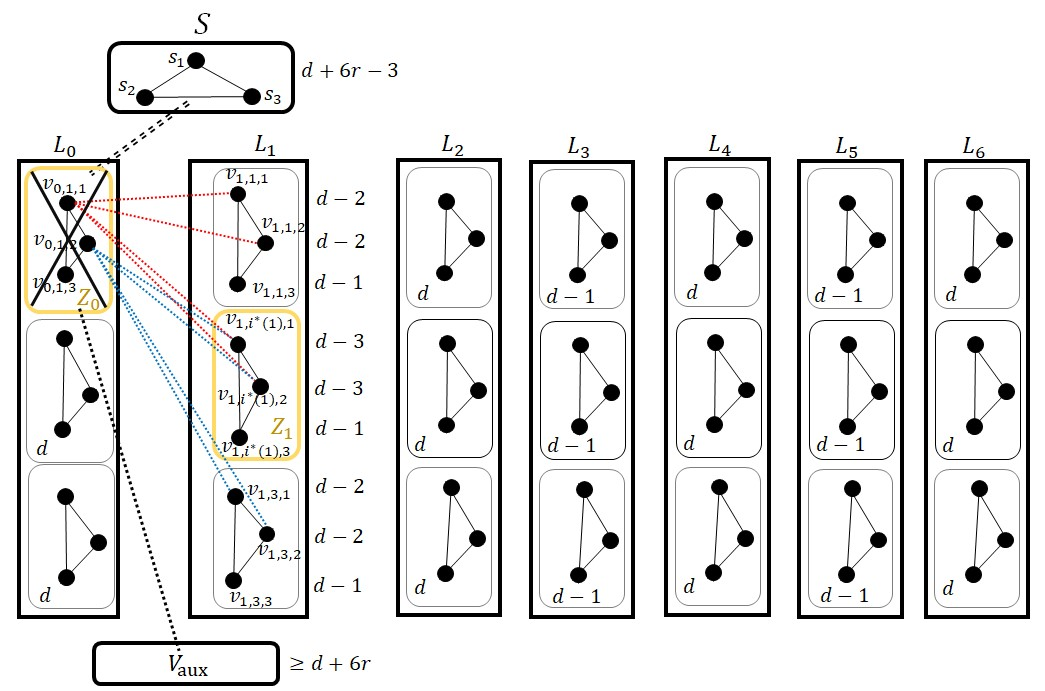
\includegraphics[width=0.65\textwidth, height=6cm]{figures/fig2}
\caption{\small The status of the graph just before iteration $4$. $Z_0$ was deleted in the last three iterations, and hence crossed out. The dotted lines denote edges that were deleted as a result. A double dotted-line between two sets of nodes signifies that originally all cross edges were present between them. Next to a node, its current degree is given. If all nodes in a set have the same degree, the value is given next to the set.}
\label{fig:first-iter}
\end{figure}

\begin{figure}[H]
\centering
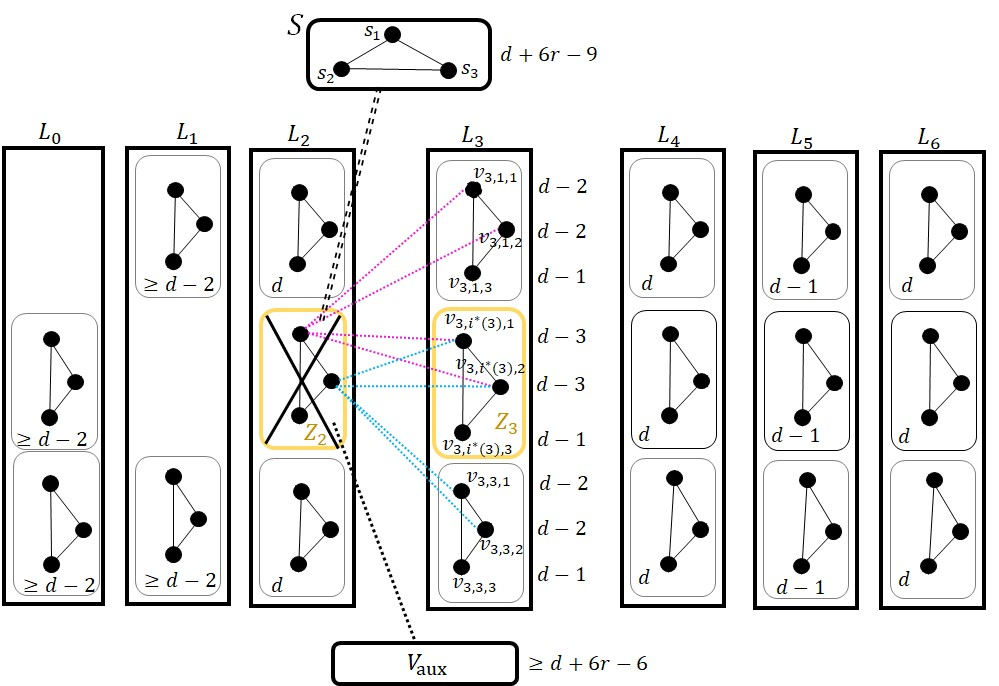
\includegraphics[width=0.65\textwidth, height=6cm]{figures/fig4}
\caption{\small The status of the graph just before iteration $10$. $Z_2$ was deleted in the last three iterations, and hence crossed out. The dotted lines denote edges that were deleted as a result. A double dotted-line between two sets of nodes signifies that originally all cross edges were present between them. Next to a node, its current degree is given. If all nodes in a set have the same degree, the value is given next to the set.}
\label{fig:even-layer-rem}
\end{figure}

 We check which nodes are affected by the removal of $Z_{\ell}$. In the original graph, the only neighbors of $Z_{\ell}$ in layer $L_{\ell-1}$ (if exists)  were the nodes in $Z_{\ell-1}$, which were removed even before $Z_\ell$ (by IH Inv.~(4)). Thus, its only neighbors in the current graph are in layer $L_{\ell+1}$, $S$, or $\Vaux$. 
 
 Suppose $\ell$ is of the form $4a+2$ (see \Cref{fig:even-layer-rem}). Then the nodes in layer $\ell+1$ represent elements in $\cX$. Recall that $Z_{\ell}$ corresponds to the element $z_{\ell'}\in \cY$ where $\ell'=\ell/2$. By construction, the edges from $Z_{\ell}$ connect to nodes that represent elements in $C_{z_{\ell'}}^{\ell'+1}$ and $D_{z_{\ell'}}^{\ell'+1}$. Consider any $x_i\in \cX$. We have three cases: (i) $x_i$ is in exactly one of the sets $C_{z_{\ell'}}^{\ell'+1}$ and $D_{z_{\ell'}}^{\ell'+1}$, (ii) $x_i$ is in neither of them, and (iii) $x_i$ is in both, i.e., $x_i=z_{\ell'+1}$. If $\ell$ is of the form $4a$ (see \Cref{fig:first-iter}), we make the analogous arguments replacing $\cX$ by $\cY$, $C$ and $D$ by $A$ and $B$, and $x_i$ by $y_i$. We now analyze each of these cases. 
 
 By IH Inv.~2(c), before iteration $3\ell+1$, each node in the triple $(v_{\ell+1,i,1}, v_{\ell+1,i,2}, v_{\ell+1,i,3})$ had degree $d-1$. Therefore, after the removal of $Z_\ell$, i.e., just before iteration $3(\ell+1)+1$, it can have the following degrees. In case (i), the triple has degrees $(d-2, d-2, d-1)$. This is because our construction ensures that exactly one of the vertices $v_{\ell,i^*(\ell),1}$ and $v_{\ell,i^*(\ell),2}$ had edges to both $v_{\ell+1,i,1}$ and $v_{\ell+1,i,2}$, and the other had none. In case (ii), it has degrees $(d-1,d-1,d-1)$. This is because none of the nodes in $Z_{\ell}$ had any edge to the triple representing $x_i$. In case (iii), the triple representing $x_i$ is precisely the triple $Z_{\ell+1}$ and has degrees $(d-3,d-3,d-1)$. This follows since both nodes $v_{\ell,i^*(\ell),1}$ and $v_{\ell,i^*(\ell),2}$ had edges to both $v_{\ell+1,i,1}$ and $v_{\ell+1,i,2}$. 
 
 The above analysis immediately implies that Inv.~3(a) holds for $\ell+1$. Now, for possible values of $r$, consider nodes in $L_r$. For $r=\ell+1$, we see that any node $v\not\in Z_{\ell+1}$ in layer $L_r$ has degree $\geq d-2$. For $r\leq \ell-1=(\ell+1)-2$, by IH Inv.~2(b), a vertex in $L_r$ had degree $\geq d-2$ before iteration $3\ell+1$, which still holds after iteration $3\ell+3$: this is because, as noted above, removal of $Z_{\ell}$ does not affect any of them. Therefore, Inv.~3(b) also holds for $\ell+1$. 
 
 For an odd $j\geq \ell+3=(\ell+1)+2$, by IH Inv.~2(c), any vertex in $L_j$ had degree $d-1$ before iteration $3\ell+1$ and it is still true after iteration $3\ell+3$ since removal of $Z_{\ell}$ cannot affect them. Thus, Inv.~3(c) holds for $\ell+1$. Finally, for an even $j\geq \ell=(\ell+1)-1$, by IH Inv.~2(d), any vertex $v\not\in Z_\ell$ had degree $d$ before iteration $3\ell+1$; since removal of $Z_{\ell}$ doesn't affect the other vertices in these layers, their degrees still have that value and Inv.~3(d) holds for $\ell+1$. Therefore, we have shown that Inv.~(3) holds for $\ell+1$.

  It remains to prove Inv.~(4). Since Inv.~(3) holds for $\ell+1$, we know that just before iteration $3(\ell+1)+1$, the triple $Z_{\ell+1}$ has degrees $(d-3,d-3,d-1)$, and any other node has degree at least $d-2$. This means the min-degree nodes in the current graph are in $Z_{\ell}$; precisely, they are $v_{\ell,i^*(\ell),1}$ and $v_{\ell,i^*(\ell),2}$, each having degree $d-3$. WLOG, say iteration $3\ell+1$ deletes $v_{\ell,i^*(\ell),1}$. Then, $\deg(v_{\ell,i^*(\ell),2})$ drops to $d-4$, and $\deg(v_{\ell,i^*,3})$ drops to $d-2$. Notice that the only other nodes that can be affected by the deletion are in either layer $L_\ell$ or layer $L_{\ell+2}$. By Inv.~3(d) for $\ell+1$, since any node in these layers had degree $d$ before iteration $3(\ell+1)+1$, their degree can drop to at least $d-1$ after the iteration. Also by Inv.~3, the vertices in other layers had degrees $\geq d-2$ before the iteration, and since they are unaffected, their degrees remain so. Hence, the current graph has the unique min-degree node $v_{\ell,i^*,2}$, which is removed by iteration $3\ell+2$. Now, $\deg(v_{\ell,i^*,3})$ drops to $d-3$. But degrees of vertices in layers $L_{\ell}$ or $L_{\ell+2}$ can now drop to at least $d-2$, while any other node maintains degree $\geq d-2$ as it's unaffected by the deletion. Hence, $v_{\ell,i^*,3}$ is the unique min-degree node in the current graph and is removed by iteration $3(\ell+1)+2$. Also observe that when each vertex was peeled, its degree was $\leq d-3$. Thus, we have proven that Inv.~(4) holds for $\ell+1$. 


\mypar{Case 2: $\ell+1$ is even} We need to show that Invs.~(2) and (4) hold for $\ell+1$. Inv.~(3) holds vacuously.  





 We know that $\ell$ is odd, and by IH, Invs.~(3) and (4) hold for $\ell$. Analgous to the last case, by Inv.~(3), we know the situation before iteration $3\ell+1$, and by Inv.~(4), we know that the iterations $(3\ell+1,3\ell+2,3\ell+3)$ remove $Z_{\ell}$, leading to the current graph just before iteration $3(\ell+1)+1$ (see \Cref{fig:odd-layer-rem} for an example with $\ell=1$ for the graph in \Cref{fig:graph-const}). 

\begin{figure}[H]
\centering
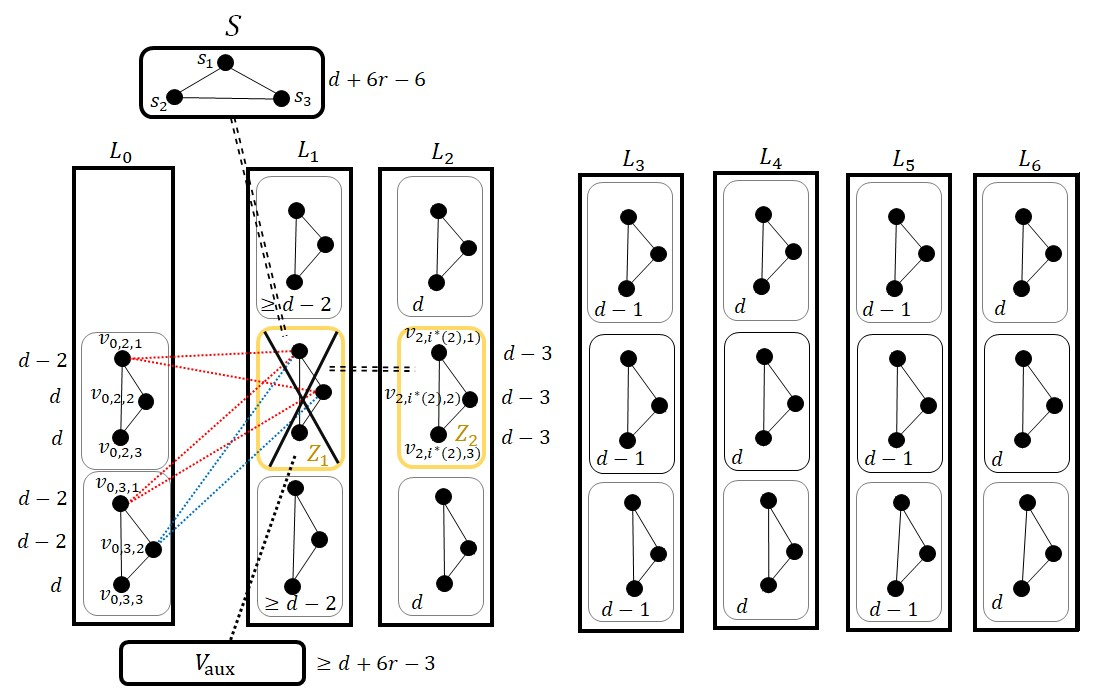
\includegraphics[width=0.65\textwidth, height=6cm]{figures/fig3}
\caption{\small The status of the graph just before iteration $7$. $Z_1$ was deleted in the last three iterations, and hence crossed out. The dotted lines denote edges that were deleted as a result. A double dotted-line between two sets of nodes signifies that originally all cross edges were present between them. Next to a node, its current degree is given. If all nodes in a set have the same degree, the value is given next to the set.}
\label{fig:odd-layer-rem}
\end{figure}


We check which nodes might be affected by the deletion of $Z_{\ell}$ in the last three iterations. By construction, $Z_{\ell}$ has edges to $Z_{\ell+1}$, to some vertices in $L_{\ell-1}$, to $S$, or to $\Vaux$. 

First consider vertices in $Z_{\ell+1}$. By IH Inv.~3(d), these nodes had degree $d$ before iteration $3\ell+1$. Further, all of them were adjacent to each node in $Z_\ell$. Hence, after $Z_{\ell}$ gets deleted, i.e., just before iteration $3(\ell+1)+1$, each of them has degree $d-3$. This shows that Inv.~2(a) holds for $\ell+1$. 

 Now consider the nodes in layer $L_{\ell-1}$. Suppose $\ell$ is of the form $4a+1$. Then the nodes in $L_{\ell-1}$ represent elements in $\cX$ and those in $L_\ell$ represent elements in $\cY$. Recall that $Z_{\ell}$ corresponds to the element $z_{\ell'}\in \cY$ where $\ell'=\ceil{\ell/2}$. Consider any $x_i\in \cX$. We have three cases: (i) $z_{\ell'}$ is in exactly one of the sets $A_{x_i}^{\ell'-1}$ and $B_{x_i}^{\ell'-1}$, (ii) $z_{\ell'}$ is in neither of them, and (iii) $z_{\ell'}$ is in both, i.e., $t_{x_i}^{\ell'-1}=z_{\ell'}$. If $\ell$ is of the form $4a+3$, we make the analogous arguments exchanging $\cX$ and $\cY$, replacing $A$ and $B$ by $C$ and $D$, and $x_i$ by $y_i$. We analyze each case.
 
 By IH Inv.~3(d), the triple representing $x_i$ in layer $\ell-1$ had degree $(d,d,d)$ before iteration $3\ell+1$. After $Z_{\ell}$ is removed, the degrees of such a triple can be the following. In case (i), it becomes either $(d-2,d,d)$ or $(d,d-2,d)$ (in \Cref{fig:odd-layer-rem}, the triple $(v_{0,2,1}, v_{0,2,2}, v_{0,2,3})$ is of this type). This is because exactly one of the vertices $v_{\ell-1,i,1}$ and $v_{\ell-1,i,2}$ had edges to both $v_{\ell,i^*(\ell),1}$ and $v_{\ell,i^*(\ell),2}$, and the other had none. In case (ii), it remains $(d,d,d)$ since neither $v_{\ell-1,i,1}$ nor $v_{\ell-1,i,2}$ had any edge to $Z_{\ell}$. In case (iii), it becomes $(d-2,d-2,d)$ (in \Cref{fig:odd-layer-rem}, the triple $(v_{0,3,1}, v_{0,3,2}, v_{0,3,3})$ is of this type). This follows since both nodes $v_{\ell-1,i,1}$ and $v_{\ell-1,i,2}$ had edges to both $v_{\ell,i^*(\ell),1}$ and $v_{\ell,i^*(\ell),2}$. 
 
 For possible values of $j$, consider the nodes in layer $L_j$ before iteration $3(\ell+1)+1$. From the above analysis, for $j=\ell-1$, any node in $L_j$ has degree $\geq d-2$. Further, by IH Inv.~3(b), for $j=\ell$ or $r\leq \ell-2$, any vertex $v\not\in Z_{\ell}$ had $\deg(v)\geq d-2$ before iteration $3\ell+1$. Since these nodes cannot be affected by the removal of $Z_{\ell}$, their degrees remain so. Therefore, we have shown that any vertex in layer $L_j$ for $j\leq \ell=(\ell+1)-1$ has degree $\geq d-2$, which means Inv.~2(b) holds for $\ell+1$. 

 By IH Inv.~3(c), for an odd $r \geq \ell+2$, any vertex in $L_j$ had degree $d-1$ before iteration $3\ell+1$. Removal of $Z_{\ell}$ doesn't affect them and hence, their degrees remain so. Thus, Inv.~2(c) holds for $\ell+1$. Finally, for an even $r\geq \ell+1$, IH Inv.~3(d) says that a vertex $v$ in $L_r$ had degree $d$ before iteration $3\ell+1$. The deletion of $Z_{\ell}$ can only affect $Z_{\ell+1}$ among these nodes. So a vertex $v\not\in Z_{\ell+1}$ in $L_j$ still has degree $d$. Therefore, Inv.~2(d), and in fact, Inv.~(2) holds for $\ell+1$.

It only remains to show that Inv.~(4) golds for $\ell+1$. Since Inv.~(2) holds for $\ell+1$, we know that just before iteration $3(\ell+1)+1$, each node in $Z_{\ell+1}$ has degree $d-3$, and any other node has degree at least $d-2$. Hence, the premise of \Cref{clm:zl-del} holds with $H$ as the current graph, $U=Z_{\ell+1}$, and $\delta=d-3$. Therefore, by \Cref{clm:zl-del}, the first three iterations on $H$, i.e., iterations $(3(\ell+1)+1,3(\ell+1)+2,3(\ell+1)+3)$ delete $Z_{\ell+1}$ in some order, and during deletion, the degree of these nodes are $\leq d-3$. Hence, Inv.~(4) holds for $\ell+1$.

Thus, we have proven that all the invariants hold for $\ell+1$ irrespective of its parity. This completes the proof by induction.
\end{proof}
 
 
 

 We are now ready to prove \Cref{lem:redn-degen-yesno}.




\begin{proof}[Proof of \Cref{lem:redn-degen-yesno}]
Indeed, we have two cases.

\mypar{Case 1: \boldmath{$b(z_r)=0$}} We show that the min-degree peeling algorithm must peel a vertex of degree $\geq d-2$ at some iteration. Then, \Cref{fact:peelingmin-degen} implies that $\kappa(G)$ must be at least $d-2$. 

\begin{figure}[H]
    \centering
    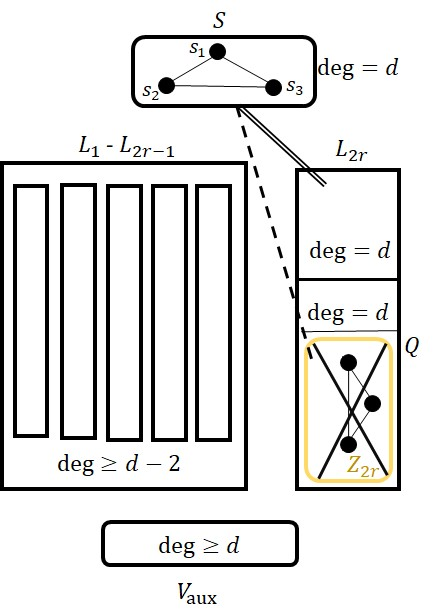
\includegraphics[scale=0.5]{figures/fig6}
    \caption{\small The graph after iteration $6r+3$ for the case $b(z_r)=0$. A double line between two sets of nodes signifies that all possible cross edges are present between them. A dashed line denotes that no edge is present between them.}
    \label{fig:nocase}
\end{figure}

    By \Cref{lem:redn-inv} Inv.~(4), the first $6r+3$ iterations of the peeling algorithm remove all the nodes in $Z_0, Z_1,\ldots, Z_{2r}$. Consider the status of the graph after $Z_{2r}$ is removed (see \Cref{fig:nocase}).  By the same lemma, all nodes in layers $L_0,\ldots, L_{2r}$ had degree $\geq d-2$ before $Z_{2r}$ was removed (i.e., just before iteration $6r+1$). Since its removal cannot affect any of those nodes
    (in these layers it only had edges to $Z_{2r-1}$, which was previously removed), their degrees remain so. Now consider nodes in $S$. By \Cref{lem:redn-inv} Inv.~1, just before iteration $6r+1$, each of them
    had degree $d$. After the next $3$ iterations remove $Z_{2r}$, their degrees remain $d$; this is because they were not connected to $Z_{2r}$ as $b(z_r)=0$. Again, by the same invariant, just before iteration $6r+1$, the nodes in $\Vaux$ had degree $\geq d+3$. Hence, after iteration $6r+3$, they must have degree $\geq d$. Therefore, the min-degree node in the current graph has degree $\geq d-2$, implying that iteration $6r+4$ of the peeling algorithm must peel a node of degree $\geq d-2$. 


\mypar{Case 2: \boldmath{$b(z_r)=1$}} Define the ordering $\sigma$ of nodes in $G$ as follows. It agrees with the order in which the min-degree peeling algorithm peels the nodes until iteration $6r+6$. Next, $\sigma$ contains the chunk of the remaining nodes in layers $L_0,\ldots,L_{2r-1}$. They are followed by the remaining nodes in layer $L_{2r}$. Finally we place the auxiliary nodes $\Vaux$. The vertices in each of these last three chunks can be placed in any arbitrary order within the chunk. We show that $\odeg_{\sigma}(v)\leq d-3$ (see \Cref{def:odegordering}) for each $v$.

\begin{figure}[H]
    \centering
    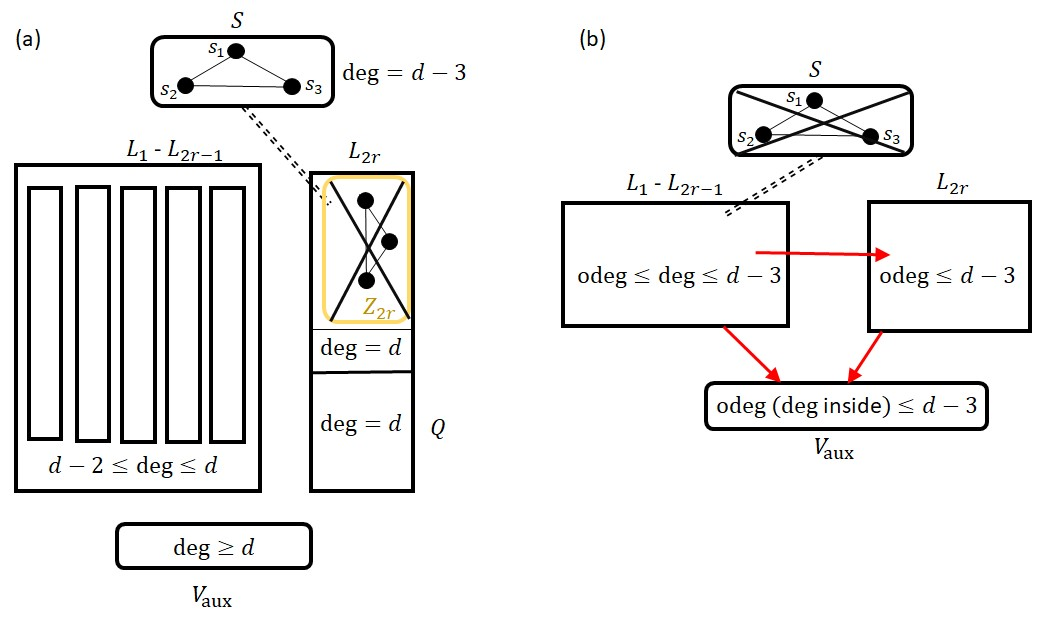
\includegraphics[scale=0.5]{figures/fig5}
    \caption{\small For the case $b(z_r)=1$: (a) the graph after iteration $6r+3$. $Z_{2r}$ was deleted in the last three iterations and hence crossed out. (b) The oriented red edges show a $(d-3)$-ordering of the nodes remaining after iteration $6r+6$. A dotted double line between two sets signifies that originally all cross edges were present between them.}
    \label{fig:yescase}
\end{figure}

As in the last case, by Inv.~(4) of \Cref{lem:redn-inv}, the first $6r+3$ iterations of the peeling algorithm remove all nodes in $Z_0,Z_1,\ldots,Z_{2r}$. Further, each time such a node is removed, its degree in the remaining graph is at most $d-3$. Again, by Inv.~(1), just before iteration $6r+1$, the nodes in $S$ had degree $d$. When the next $3$ iterations remove $Z_{2r}$ (see \Cref{fig:yescase}(a)), their degrees drop to $d-3$ this is because all nodes in $S$ were adjacent to all nodes in $Z_{2r}$ as $b(z_r)=1$. By the invariants in \Cref{lem:redn-inv}, all other remaining nodes have degree $\geq d-2$. Hence, the premise of \Cref{clm:zl-del} applies with $H$ as the current graph, $U=S$, and $\delta=d-3$. By \Cref{clm:zl-del}, the first three iterations on $H$, i.e., iterations $(6r+4,6r+5,6r+6)$ remove the nodes in $S$, each having degree $\leq d-3$ when deleted. Since $\sigma$ agrees with the peeling algorithm until this iteration, and we showed that every vertex $v$ until now has been removed while having degree $\leq d-3$, it follows that $\odeg_{\sigma}(v)\leq d-3$ for each such $v$. 

After $S$ is removed (see \Cref{fig:yescase}(b)), observe that all remaining nodes in layers $L_0,\ldots,L_{2r-1}$ have degree $\leq d-3$ since they had degree $\leq d$ before the removal of $S$, and they were all adjacent to all three nodes in $S$. Hence, regardless of their order in $\sigma$, $\odeg_{\sigma}(v)\leq d-3$ for any such node $v$. If we remove these nodes from the graph, then each node in layer $L_{2r}$ will have degree $\leq d-3$ in the remaining graph: it initially had degree $d$, and now has lost at least its $3$ neighbors in layer $L_{2r-1}$. Thus, $\odeg_{\sigma}(v)\leq d-3$ for each such node $v$. 

Finally, the auxilary nodes $\Vaux$ remain, and by \Cref{lem:redn-aux-constr}, the induced subgraph $G[\Vaux]$ has degree $\leq d-3$. Therefore, $\odeg_{\sigma}(v)\leq d-3$ for any $v\in \Vaux$ and we conclude that $\odeg_{\sigma}(v)\leq d-3$ for all $v\in V$. Hence, $\sigma$ is a $(d-3)$-ordering of vertices in $G$. Then by \Cref{fact:min-k-ord}, we get that $\kappa(G)\leq d-3$.
\end{proof}




\subsection{Completing the Reduction: Streaming to Communication Protocol}
We now put things together and complete the reduction to prove \Cref{thm:degen-lb}. We restate the theorem here. 

\mainthmdegen*


\begin{proof}
Suppose there is a $p$-pass $S$-space streaming algorithm $\cA$ that, given an integer $k$, outputs YES if $\kappa(G)\leq k$ and NO if not. Then, given an instance of $\bmhpc_{m,2p-1}$, the players $P_A, P_B, P_C,$ and $P_D$ run the following $(2p-1)$-phase protocol. They collectively feed the graph $G=(V,E)$ as in \Cref{lem:redn-aux-constr} to $\cA$ as follows. 

First note that the vertex set $V$ is known to all the players. Further, the edge sets $E_1,E_2,E_S$ are also input-independent and known to all players. In phase $1$ of the protocol, $P_C$ starts pass $1$ of the algorithm $\cA$ and inserts the edges in these sets. She then adds the edges $E_C$ which are completely determined by her input. Next, she sends the current state of $\cA$ along with all the vertex-degrees in the current graph to $P_D$. The player $P_D$ continues the stream by adding the edges in $E_D$, which is determined by his input. Next, he sends the current state of $\cA$ along with the updated vertex-degrees of the current graph (which he can calculate from the edges he added and the information sent to him by $P_C$) to the player $P_A$. This ends phase $1$.

In phase $2$, $P_A$ further extends the stream by adding the edges in $E_A$, which is given by her input. She sends the algorithm's state along with the updated node-degrees to $P_B$. The player $P_B$ adds the edge set $E_B$ and updates the degrees. Observe that the current graph has the edge set $E'$ as defined above. From the degree information, $P_B$ can now determine the edges $\Eaux$ to be added to set the target node-degrees (by \Cref{lem:redn-aux-constr}). Hence, $P_B$ adds those edges, which completes the first pass of $\cA$ on $G$. To end phase $2$, $P_B$ sends the current state of the algorithm to $P_C$. In phase $3$, $P_C$ starts pass $2$ of the algorithm by inserting the same edges that she added in phase $1$. They repeat the protocol as before for pass $2$, except that they no longer communicate degree information since $P_B$ already knows $\Eaux$. Thus, the players can simulate one pass of $\cA$ using two phases of the communication protocol, except the last pass that requires just one phase. After the final pass of $\cA$, the player $P_B$ looks at the output given by the algorithm for $k = d-3 = 6m(2p-1)+3m-3$ and determines the answer to $\bmhpc_{m,2p-1}$ (using \Cref{lem:redn-degen-yesno}). 

Thus, the players can solve $\bmhpc_{m,2p-1}$ using $2p-1$ phases and $O(pS+n\log n)$ bits of communication. By \Cref{thm:lb-mhpc}, it follows that $pS\geq \Omega(m^2- n\log n)$. Since $n=\Theta(mp)$ by \Cref{lem:redn-aux-constr}, we get that $pS\geq \Omega(n^2/p^2 - n\log n)$, which implies that $S\geq \Omega(n^2/p^3 - (n\log n)/p)$. This completes the proof of the theorem.  \end{proof}

We observe that the reductions for lexicographically-first maximal independent set (LFMIS) and s-t min-cut from \hpc in \cite{AssadiCK19} have a similar layered graph, where the \emph{same} \hpc instance is repeated between alternate pairs of consecutive layers. Instead, we can reduce from \mhpc as follows: similar to our reduction for degeneracy, we can make the successive pairs of layers encode the \emph{distinct} ``instances'' of \hpc that are given in a single instance of \mhpc. Then, following very similar arguments as above, the reductions from \mhpc to these problems go through and their streaming lower bounds are improved. Thus, we can prove \Cref{cor:lfmis-mincut}. We skip the formal details. 

